% Notizen

\chapter{Notizen} % Main chapter title

\label{Notizen} % For referencing the chapter elsewhere, use \ref{Chapter1} 

%----------------------------------------------------------------------------------------

% Define some commands to keep the formatting separated from the content 
%\newcommand{\keyword}[1]{\textbf{#1}}
%\newcommand{\tabhead}[1]{\textbf{#1}}
%\newcommand{\code}[1]{\texttt{#1}}
%\newcommand{\file}[1]{\texttt{\bfseries#1}}
%\newcommand{\option}[1]{\texttt{\itshape#1}}


%----------------------------------------------------------------------------------------

\section{C-Nets}

Causal nets (C-nets) -> a tuple $(\Sigma, s_i , s_o , D, I, O)$\\

\begin{itemize}
\item{$\Sigma$ endliches Set an Aktivitäten}
\item{$s_i \in \Sigma$ eindeutige Start Aktivität}
\item{$s_o \in \Sigma$ eindeutige Ende Aktivität}
\item{$D \subseteq \Sigma \times \Sigma$ Abhängigkeitsbeziehung}
\item{$B = \{X \subseteq \mathscr{P} (\Sigma) \; \rvert \; X = \{ \varnothing \} \vee \varnothing \notin X \} $  mögliche Bindunge}
\item{$I \in \Sigma \rightarrow B$ Set der Input Bindungen pro Aktivität}
\item{$O \in \Sigma \rightarrow B$ Set der Output Bindungen pro Aktivität}

\end{itemize}
%--------------------------------------------------------------------------------------


\pagebreak
\section{ProM Schulung}

\begin{figure}[H]
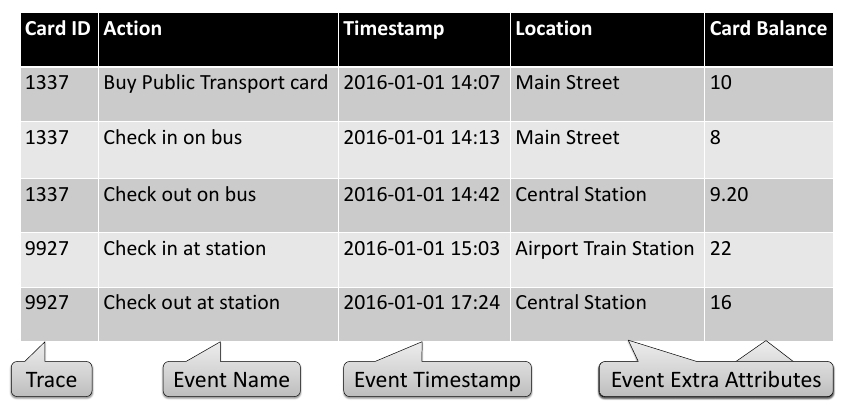
\includegraphics[width=14cm]{Chapters/Notizen_Graphics/TransportEventData.jpg}
\caption{Eventdaten eines Transportprozesses} 
\end{figure}

\begin{figure}[H]
\vspace*{.04\textheight}
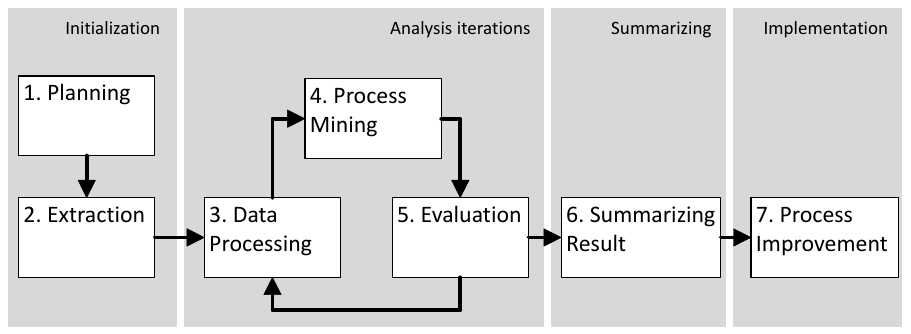
\includegraphics[width=14cm]{Chapters/Notizen_Graphics/ProcessMiningSteps.jpg}
\caption{Schritte des Process Mining} 
\end{figure}

\subsection{Petrinets}

\textbf{Petrinet Notation}
\begin{figure}[H]

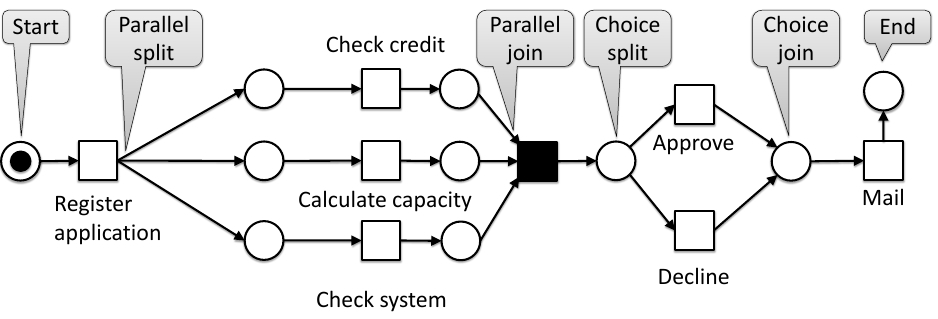
\includegraphics[width=14cm]{Chapters/Notizen_Graphics/Petri_Notation.jpg}
\caption{Petrinets Notation} 
\end{figure}

\begin{figure}[H]
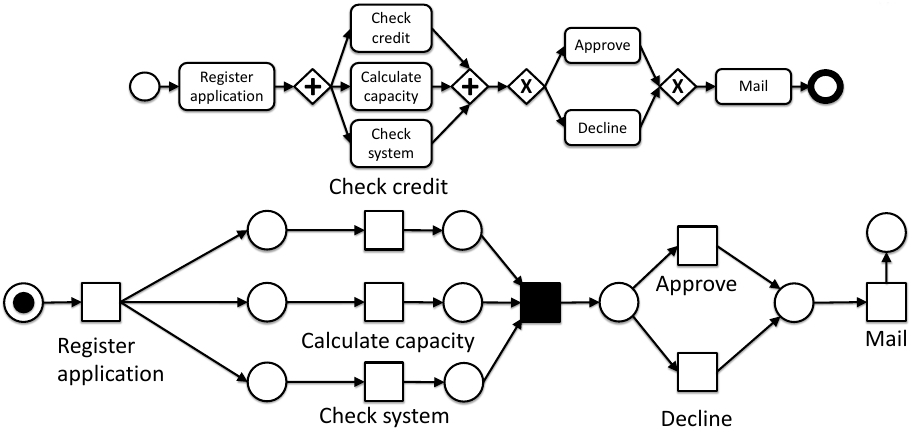
\includegraphics[width=14cm]{Chapters/Notizen_Graphics/Petri_BPMN_Notation.jpg}
\caption{Petrinets Notation vgl. mit BPMN} 
\end{figure}


\subsection{Recognize Patterns}
The goal is to discover a process model from event logs.
After the discovery follow conformance and enhancement as process mining procedures.

\begin{figure}[H]
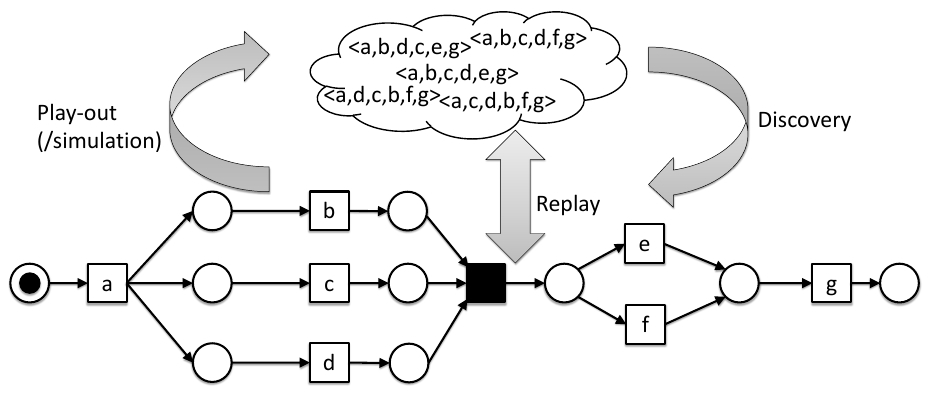
\includegraphics[width=14cm]{Chapters/Notizen_Graphics/ProcessModel_Behaviour.jpg}
\caption{Ableitung des Petrinets aus Eventlogs} 
\end{figure}

Common patterns:
\begin{itemize}
\setlength{\itemsep}{0.4mm}
\item{Sequence}
\item{Choice}
\item{Parallelism}
\item{Loops}
\end{itemize}

\begin{figure}[H]
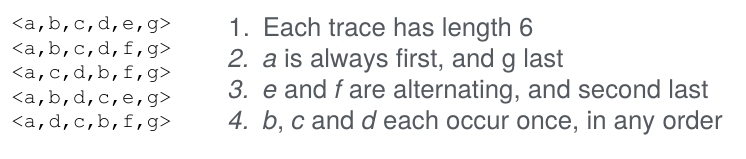
\includegraphics[width=14cm]{Chapters/Notizen_Graphics/Recognize_Patterns.jpg}
\caption{Muster in Traces erkennen} 
\end{figure}

\textbf{Detect and ignore noise}
\begin{figure}[H]
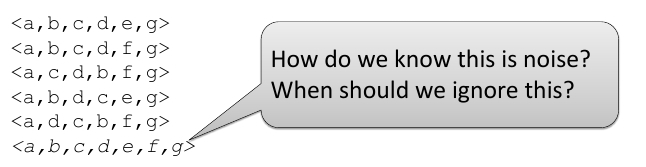
\includegraphics[width=14cm]{Chapters/Notizen_Graphics/Detect_Noise.jpg}
\caption{Hintergrundrauschen/ Noise erkennen} 
\end{figure}

\vspace{5mm}\pagebreak
\textbf{Main challenges in process discovery}
\begin{enumerate}
\setlength{\itemsep}{3pt}
\item{Discover sound process models}
\item{Recognize patterns}
\item{Detect and ignore noise}
\item{Generalize from observations}
\end{enumerate}

\vspace{5mm}
\textbf{Process model checklist}
\begin{enumerate}
\setlength{\itemsep}{3pt}
\item Soundness: Are the criterion for Soundness met?
\item Replay Fitness: Can all traces be represented by the model?
\item Precision: Can the model represent additional cases, not seen in the traces? 
\item Generalization: Is the model restrictive or can it be applied in general?
\item Simplicity: Is the model as simple as possible?
\end{enumerate}

\vspace{5mm}
\textbf{Soundness}
\begin{enumerate}
\setlength{\itemsep}{3pt}
\item{Option to complete}\\
For each possible state of the process model, it is possible to reach the end state

\item{Proper completion}\\
When the process model reaches the end state, there are no tokens left behind

\item{No dead transitions}\\
Each transition in the process model can be enabled
\end{enumerate}

\pagebreak
\section{Different Miners}
\subsection{Alpha Miner}
Very first Miner to bridge from Event Logs to Petri Nets - Mining Process Models.

\begin{enumerate}
\item Detects Footprint Matrix
\item Derives PetriNet
\end{enumerate}

\begin{figure}[H]
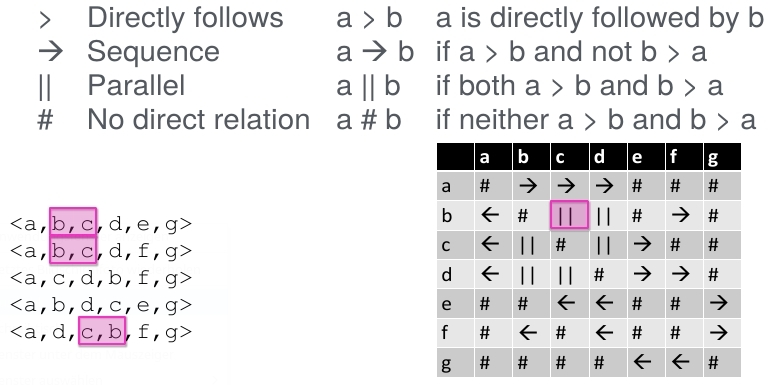
\includegraphics[width=14cm]{Chapters/Notizen_Graphics/Notation_FootprintMatrix.jpg}
\caption{Notation and the Footprint Matrix} 
\end{figure}

\begin{figure}[H]
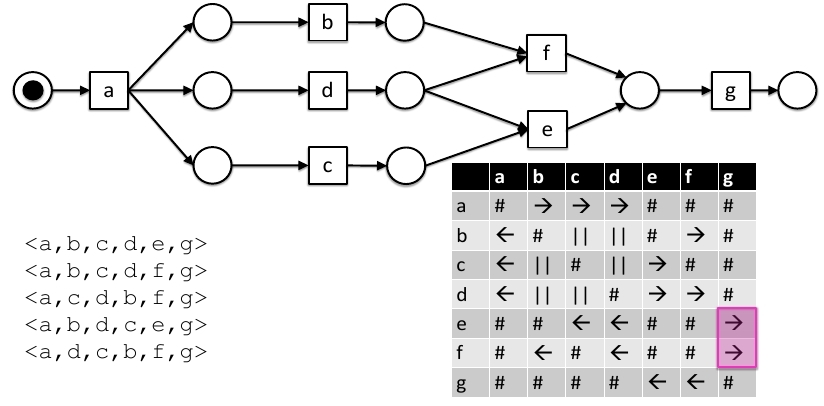
\includegraphics[width=14cm]{Chapters/Notizen_Graphics/Notation_FootprintMatrix_PetriNet.jpg}
\caption{Notation and the Footprint Matrix} 
\end{figure}

\begin{figure}[H]
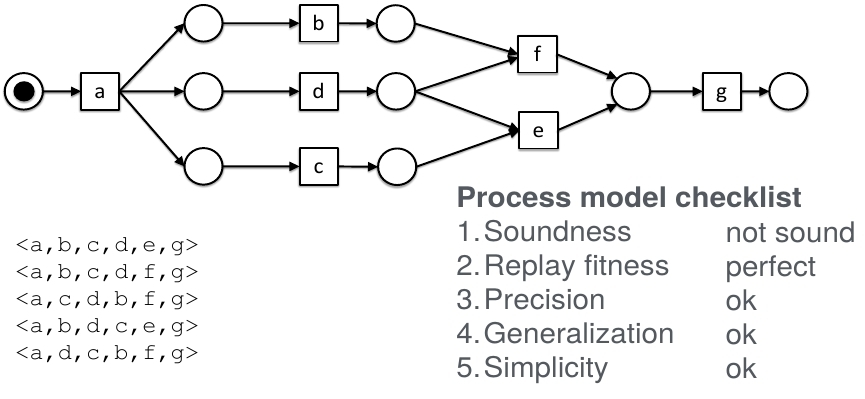
\includegraphics[width=14cm]{Chapters/Notizen_Graphics/Checklist_AlphaMiner.jpg}
\caption{Notation and the Footprint Matrix} 
\end{figure}

\section{Heuristics Miner}
\begin{itemize}
\item{Improvement of the Alpha miner}
	\begin{itemize}
	\item Takes frequencies into account
	\item Detects short-loops
	\item Detects skipping activities
	\end{itemize}
\item Does not guarantee sound process models
\end{itemize}

\begin{framed} \begin{equation}
=> = \frac{|a>b|-|b>a|}{|a>b|-|b>a|+1}
\end{equation} 
\end{framed}

\begin{figure}[H]
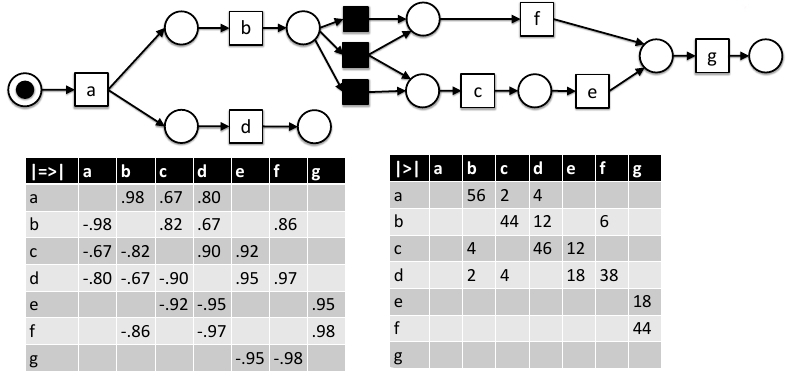
\includegraphics[width=14cm]{Chapters/Notizen_Graphics/HeuristicsMiner_Dependency_Matrix.jpg}
\caption{Dependency Matrix des Heuristic Miners} 
\end{figure}



Aus der "Frequency" rechts wird die "Significance" links berechnet. |a>b| ist die Häufigkeit in der b auf a gefolgt ist (hier 56).
-> Durch die Dependency Matrix können signifikante Abhängigkeiten erkannt werden

\begin{figure}[H]
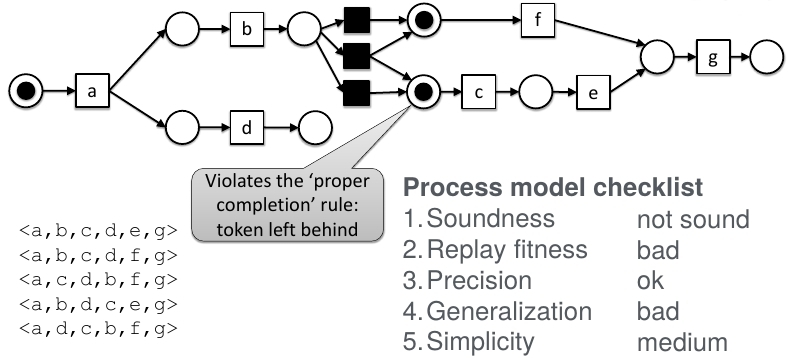
\includegraphics[width=14cm]{Chapters/Notizen_Graphics/HeuristicsMiner_conclus.jpg}
\caption{Heuristic Miner - Modell Check} 
\end{figure}


\section{Inductive Miner}
\begin{itemize}
\setlength{\itemsep}{3pt}
\item Guarantees sound process models
\item Repeatedly
	\begin{itemize}
	\item Find most prominent split in event log
	\item Detect operator
	\item Continue on both sublogs
	\end{itemize}
\end{itemize}

\begin{figure} [H]
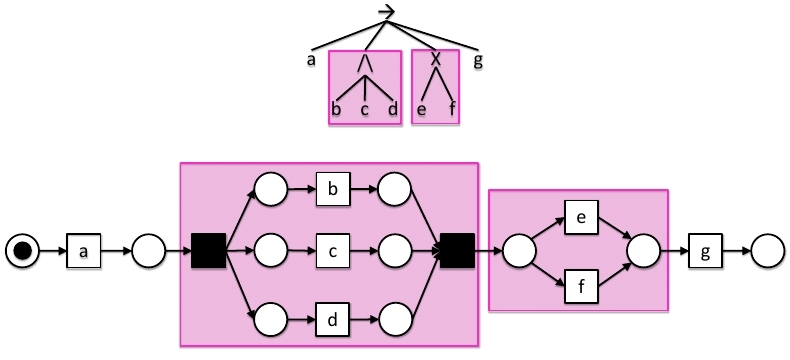
\includegraphics[width=14cm]{Chapters/Notizen_Graphics/InductMin_soundness.jpg}
\vspace*{.02\textheight}
\caption{Inductive Miner - Ableiten eines Entscheidungsbaums} 
\end{figure} 

\begin{figure} [H]
    \subfigure[Always a]{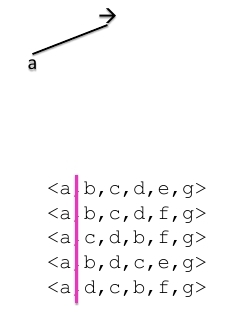
\includegraphics[width=0.34\textwidth]{Chapters/Notizen_Graphics/InductMin_repeat1.jpg}} 
    \subfigure[Always e OR f]{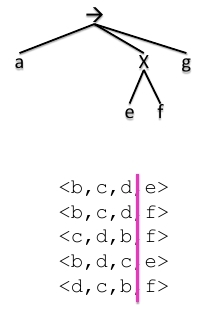
\includegraphics[width=0.3\textwidth]{Chapters/Notizen_Graphics/InductMin_repeat2.jpg}}
    \subfigure[Parallelism b,c,d]{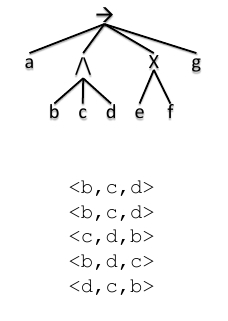
\includegraphics[width=0.33\textwidth]{Chapters/Notizen_Graphics/InductMin_repeat3.jpg}} 
\caption{Inductive Miner - Repeatedly Split Event Log} 
\end{figure} 


\begin{figure} [H]
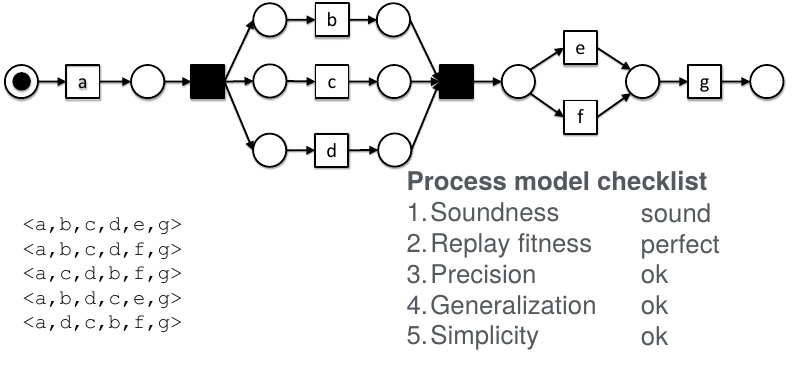
\includegraphics[width=14cm]{Chapters/Notizen_Graphics/InductMin_conclus.jpg}
\vspace*{.02\textheight}
\caption{Inductive Miner - Modell Check} 
\end{figure} 

Trennung der Traces leitet Baumstruktur und somit Modell ab.

\pagebreak
\section{Conformance Checking}
\subsection{Alignments}

Move along the trace and follow the token in the PetriNet.

\noindent\textbf{"Move on log only"}: If the arrow moved only in the trace and not in the model (i.e. f follows e in trace but not the PetriNet) the Symbol ">>" is marked down in the Model row of the Table.\\

\begin{figure} [H]
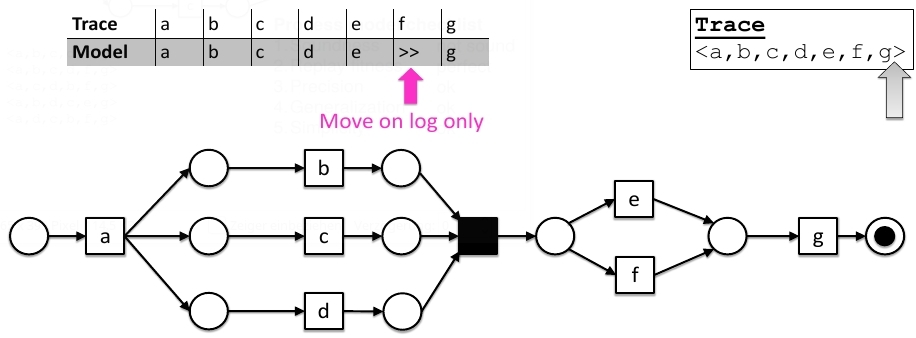
\includegraphics[width=14cm]{Chapters/Notizen_Graphics/MoveLogOnly_ConformanceCheck.jpg}
\vspace*{.02\textheight}
\caption{Compare Trace and Model} 
\end{figure} 

\textbf{This Method:}
\begin{itemize}
\item Explores multiple options to find the optimal alignment (guaranteed)
\item Allows flexible costs to activities and move types (e.g. a model move on e can be preferred over a log move on f)
\item Relates the event log to the process model and hence enables further analysis



\end{itemize}



\begin{figure} [H]
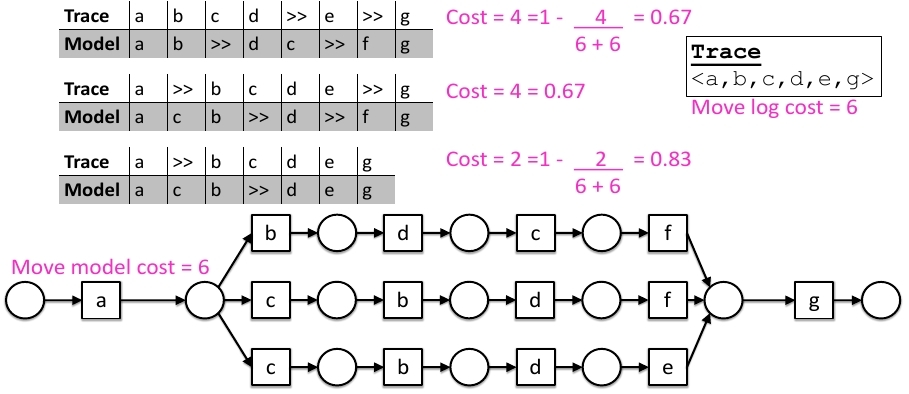
\includegraphics[width=14cm]{Chapters/Notizen_Graphics/ReplayFitness_ConformanceChecking.jpg}
\caption{Calculate Replay Fitness for each Trace} 
\end{figure} 

\begin{framed} \begin{equation}
Replay Fitness = 1 - \frac{Cost Of Allignment}{Move Log Cost + Move Model Cost}
\end{equation} 
\end{framed}


\subsection{Performance Analysis}

Normally only the \textbf{completion time} of an activity is known.\\
If the \textbf{starting time} is given as well, it is possible to distinguish between waiting and execution time. Otherwise it is only possible to calculate the time spent in one place.
\begin{figure} [H]
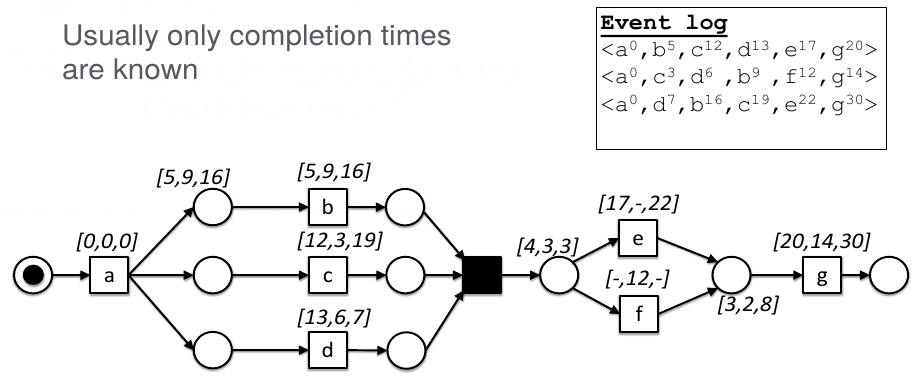
\includegraphics[width=14cm]{Chapters/Notizen_Graphics/TimestampsInTraces_PerformanceChecks.jpg}
\caption{Adding Timestamps in Traces and Modell} 
\end{figure} 


\textbf{Steps in ProM:}
\begin{itemize}
\item Load Data (here: \glqq Artificial - Loan Process.xes.gz\grqq)
\item Mine Process Model (here \glqq Mine Petri net with Inductive Miner\grqq)
\item \glqq Replay a Log on Petri nets for Performance/Conformance Analysis\grqq

\end{itemize}


\begin{figure} [H]
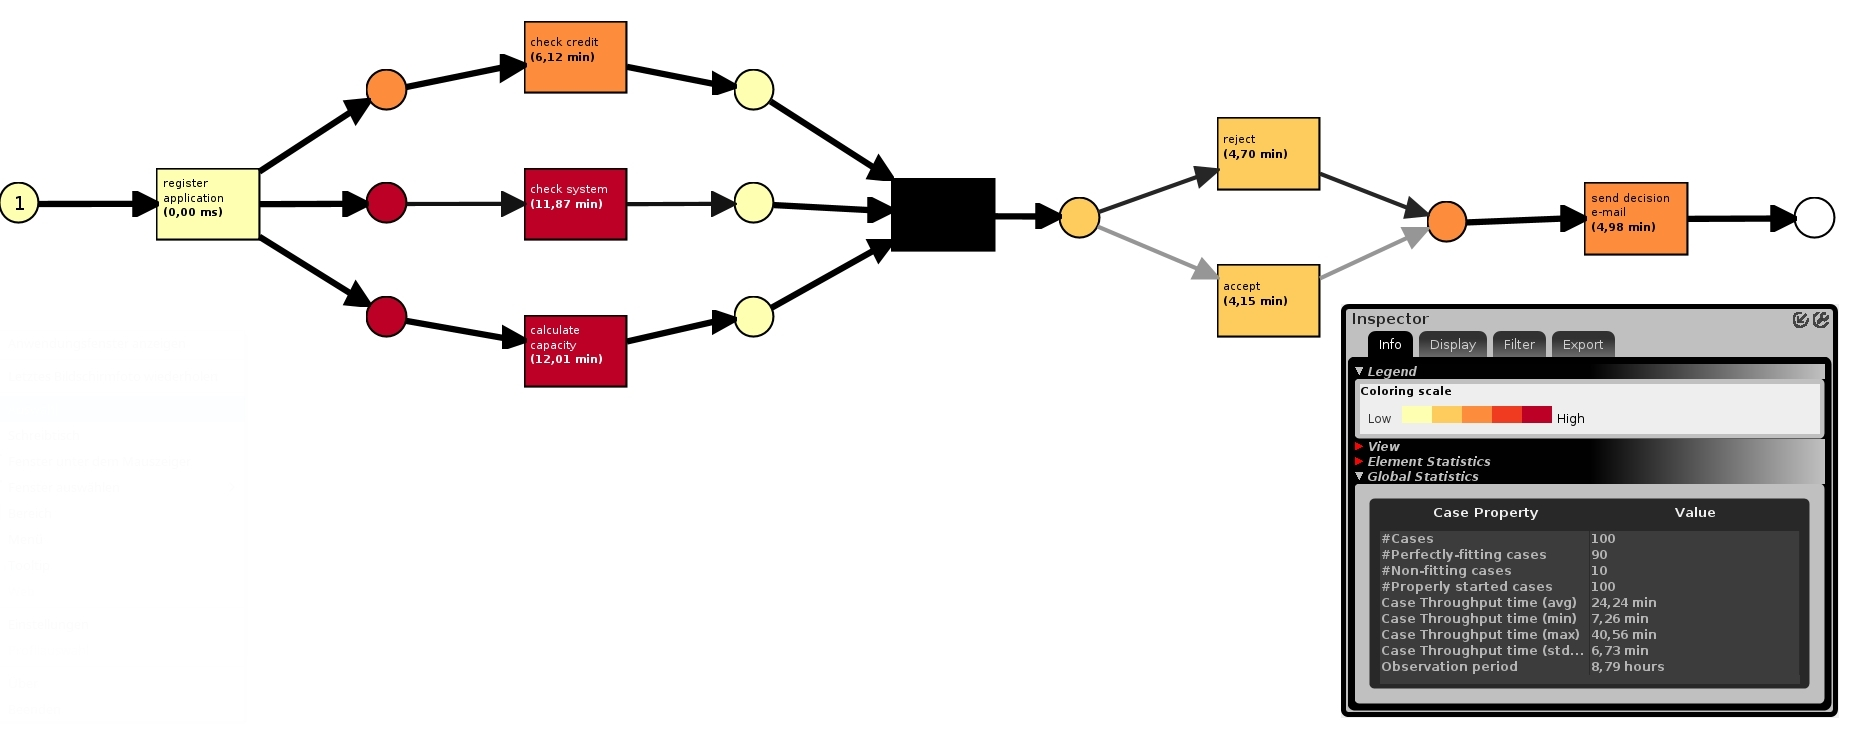
\includegraphics[width=14cm]{Chapters/Notizen_Graphics/ProM_PerformanceChecking.jpg}
\caption{Performance Checking in ProM} 
\end{figure} 

\noindent The darker red means, that the case took longer than others.\\
Question where time is spent - mainly in the parallel process, because two of them take some time and others have to wait (not sequential).\\

From the time it takes to go through certain parts of the model it might be possible to get results concerning the Conformance by analyzing deviations. (i.e. if time to complete one case is longer than average run time - possible that case is not included in every trace)


\begin{figure} [H]
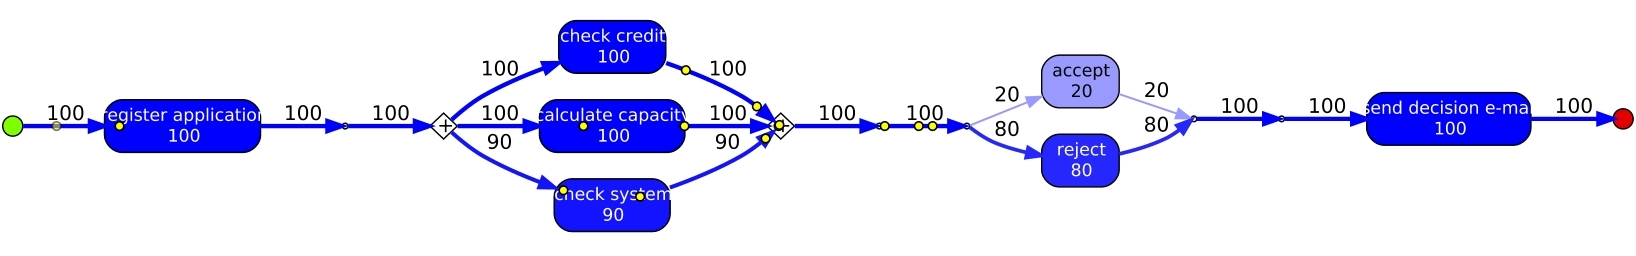
\includegraphics[width=14cm]{Chapters/Notizen_Graphics/InductiveVisualMiner_PerformanceAnalysis.jpg}
\caption{Performance Checking in ProM with the Inductive Visual Miner} 
\end{figure} 
Each transition can be seen in the graph - further 
 